\documentclass[conference]{IEEEtran}
\IEEEoverridecommandlockouts
% The preceding line is only needed to identify funding in the first footnote. If that is unneeded, please comment it out.
\usepackage{cite}
\usepackage{amsmath,amssymb,amsfonts}
\usepackage{algorithmic}
\usepackage{graphicx}
\usepackage{textcomp}
\usepackage{xcolor}
\def\BibTeX{{\rm B\kern-.05em{\sc i\kern-.025em b}\kern-.08em
    T\kern-.1667em\lower.7ex\hbox{E}\kern-.125emX}}
\begin{document}

\title{Implementation of a Two's Complement Circuit*\\
{\footnotesize \textsuperscript{*}Note: Sub-titles are not captured in Xplore and
should not be used}
\thanks{Identify applicable funding agency here. If none, delete this.}
}

\author{\IEEEauthorblockN{Nan Lin}
\IEEEauthorblockA{\textit{SPEIT} \\
\textit{Shanghai Jiao Tong University}\\
Shanghai, China \\
lns\_brandon@sjtu.edu.cn}
\and
\IEEEauthorblockN{Yanxu Meng}
\IEEEauthorblockA{\textit{SPEIT} \\
\textit{Shanghai Jiao Tong University}\\
Shanghai, China \\
email address or ORCID}
}

\maketitle

\begin{abstract}
This document is a model and instructions for \LaTeX.
This and the IEEEtran.cls file define the components of your paper [title, text, heads, etc.]. *CRITICAL: Do Not Use Symbols, Special Characters, Footnotes, 
or Math in Paper Title or Abstract.
\end{abstract}

\begin{IEEEkeywords}
component, formatting, style, styling, insert
\end{IEEEkeywords}


\section{Question 1-5}

\subsection{Question 1}

The two's complement of a binary number is obtained by inverting its digits and adding one to the least significant bit. This method allows for straightforward binary arithmetic and simplifies the design of digital circuits for arithmetic operations.

A half-adder is a fundamental component in digital arithmetic. It takes two single-bit binary inputs and produces a sum and carry output. The truth table for a half-adder is shown below:

\begin{table}[h!]
\centering
\begin{tabular}{|c|c|c|c|}
\hline
A & B & Sum & Carry \\ \hline
0 & 0 &  0  &   0   \\ \hline
0 & 1 &  1  &   0   \\ \hline
1 & 0 &  1  &   0   \\ \hline
1 & 1 &  0  &   1   \\ \hline
\end{tabular}
\caption{Truth table for a half-adder}
\end{table}

The corresponding half-adder circuit diagram is illustrated in Figure~\ref{fig:half_adder}.

\begin{figure}[h!]
\centering
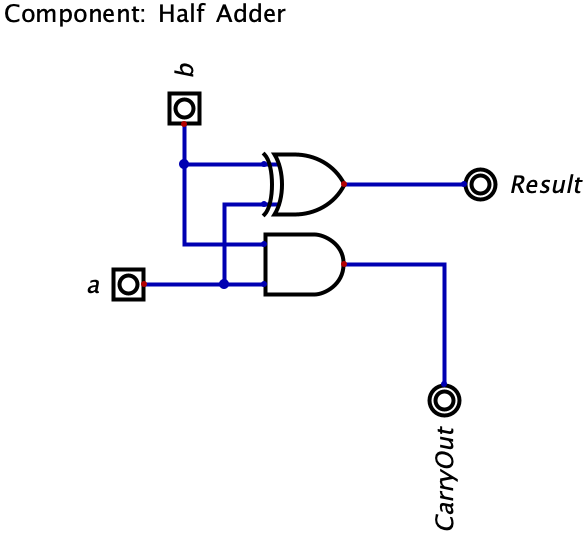
\includegraphics[width=0.5\textwidth]{assets/half_adder.png}
\caption{Half-Adder Circuit}
\label{fig:half_adder}
\end{figure}

To create an 8-bit two's complement circuit, we combine multiple half-adders. The process involves inverting each bit of the input number and then adding one using a series of adders. The detailed circuit diagram is shown in Figure~\ref{fig:twos_complement}.

\begin{figure*}[h!]
\centering
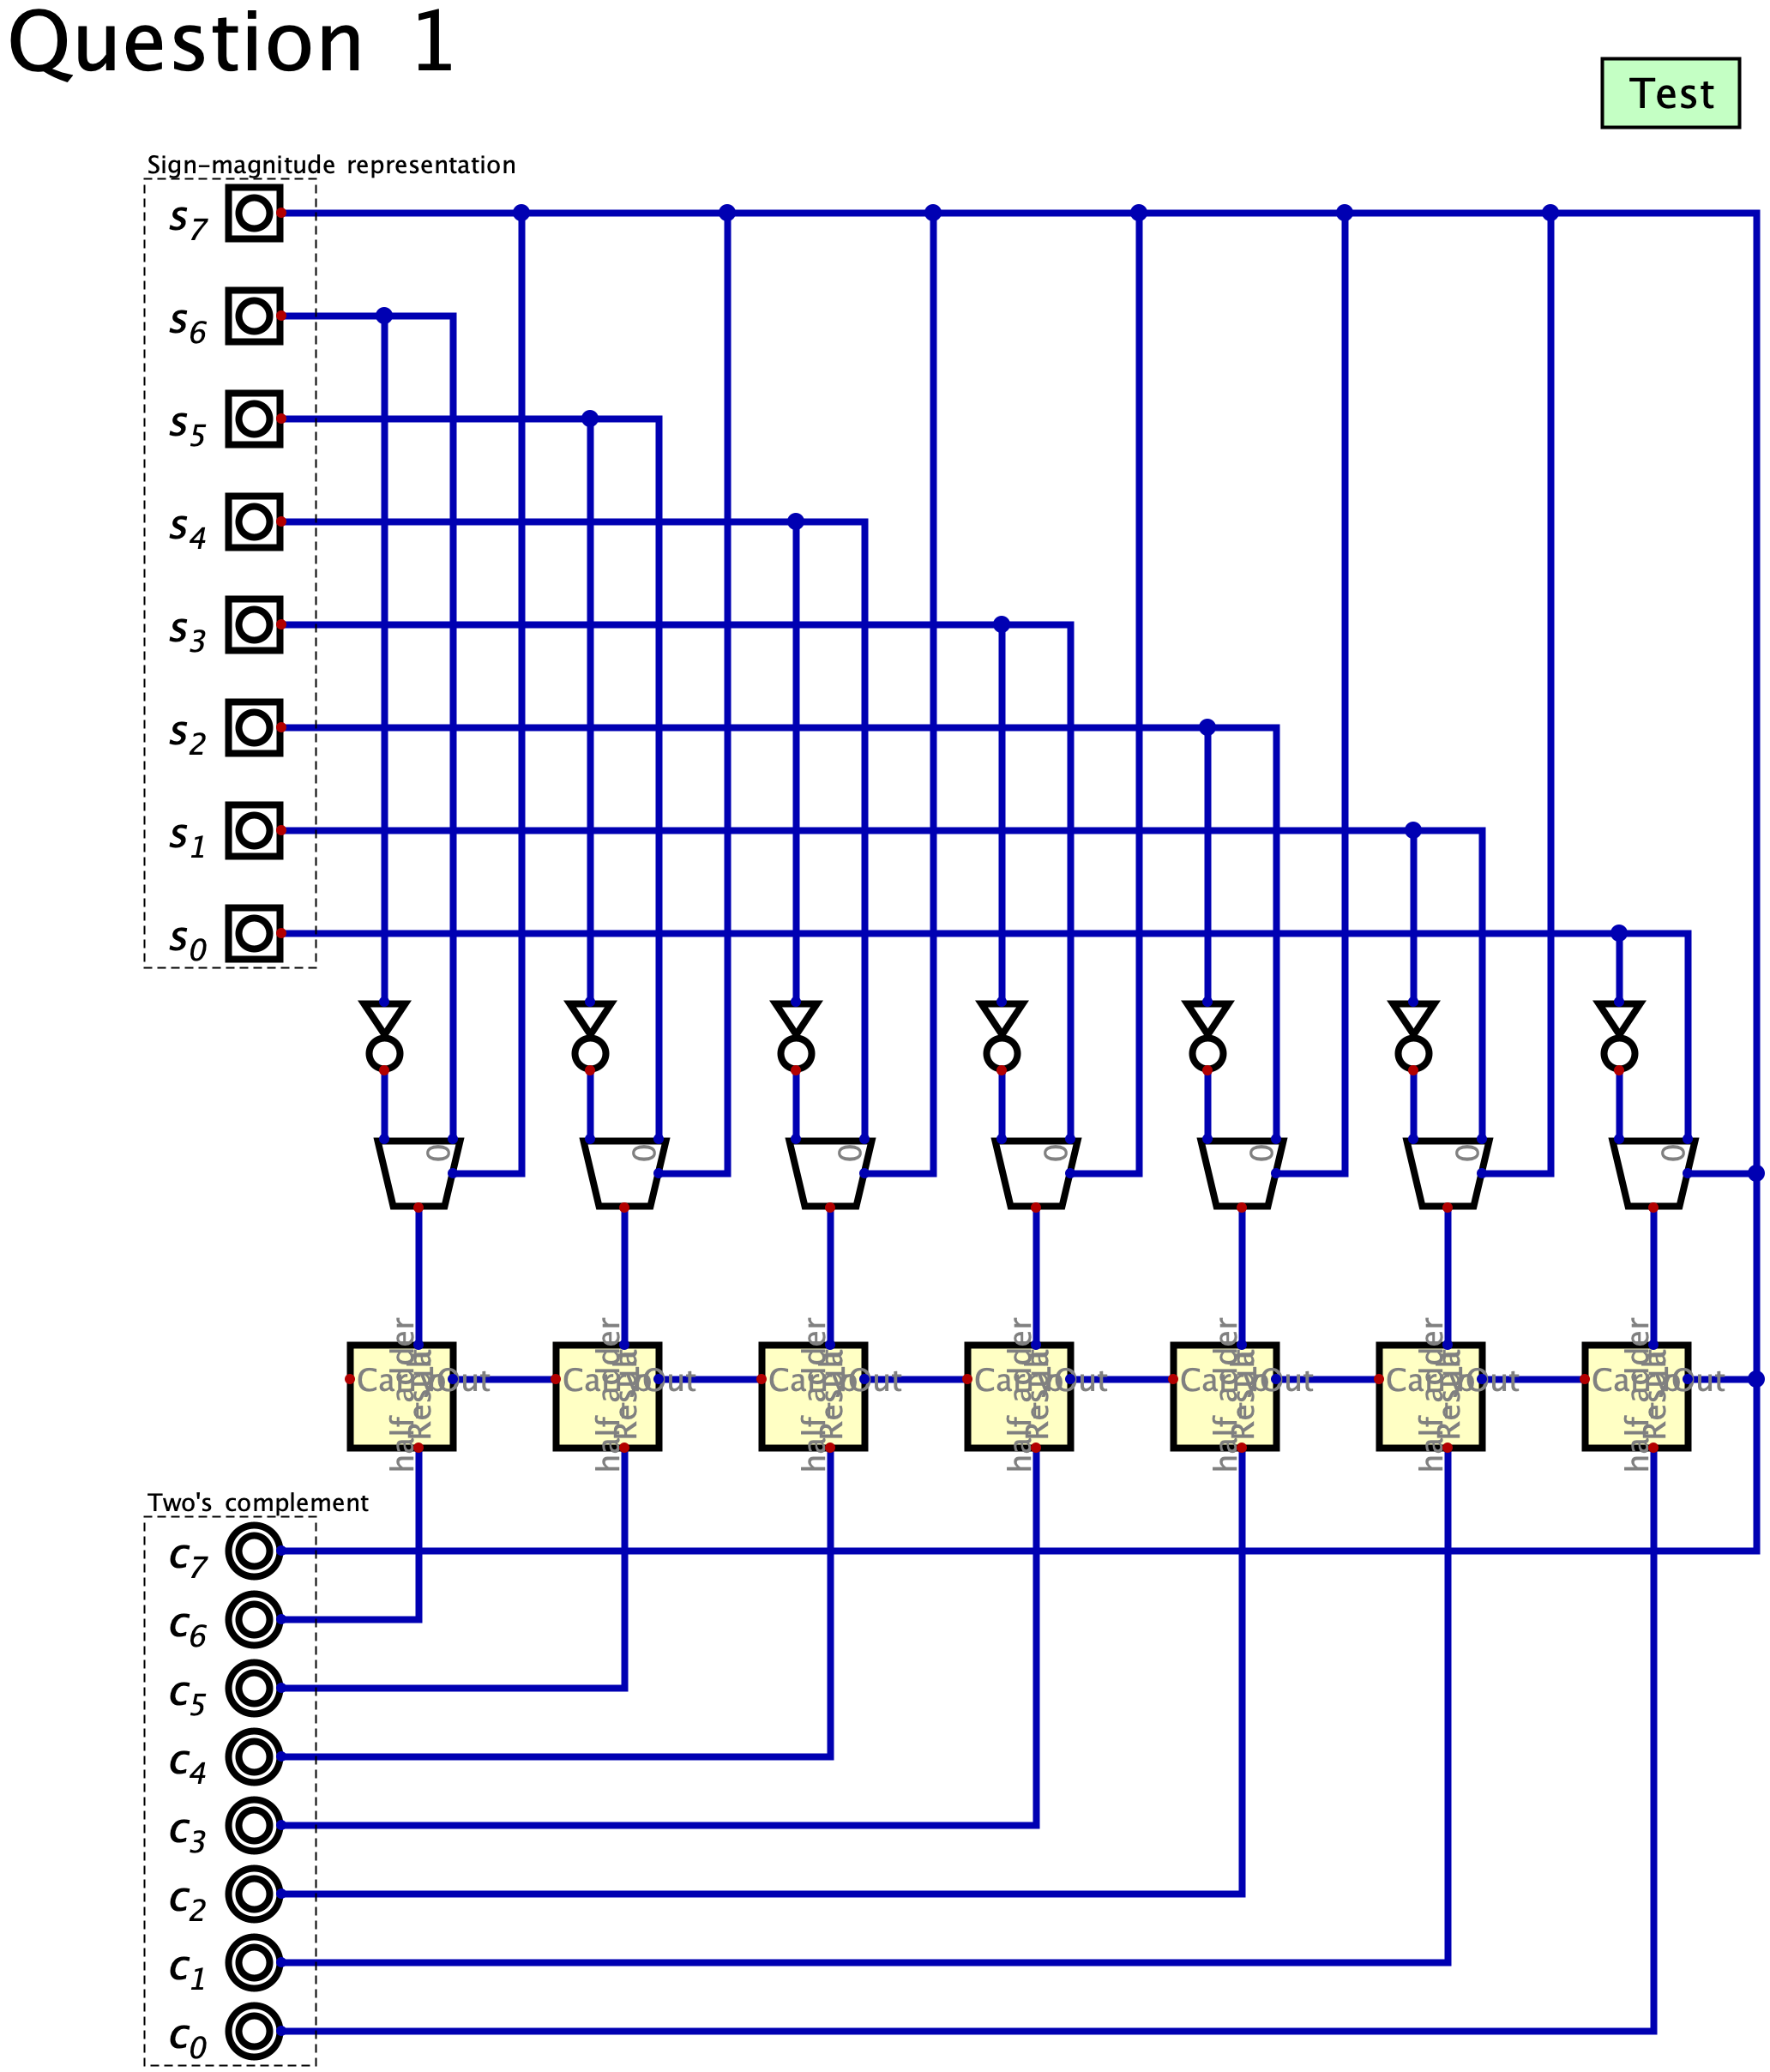
\includegraphics[width=\textwidth]{assets/twos_complement.png}
\caption{8-bit Two's Complement Circuit}
\label{fig:twos_complement}
\end{figure*}


\subsection{Question 2}

To analyze the depth and complexity of the two's complement circuit for 8 bits, we divide the process into two stages.

The first stage is the \textbf{inversion stage}. Each bit requires a NOT gate, thus:
\begin{itemize}
\item Depth: 1 (because all the NOT gates operate simultaneously)
\item Complexity: 7 (NOT gates)
\end{itemize}

The second stage is the \textbf{addition stage}. For each bit, a half-adder is applied.
The half-adder of the highest bit besides the sign bit (here, it is $c_6$) requires all the preceding adders to compute the result to operate.
Therefore, the depth is 7 and the number of gates is $2 \times (8 - 1) = 14$.

In conclusion, for an 8-bit two's complement, the depth is $1 + 7 = 8$ and the complexity is $8 + 14 = 22$.

We expand the results to any $2^p$-bit ($p \in \mathbb{N}$) two's complement circuit.

\begin{enumerate}
\item In the \textbf{inversion stage}, the depth is 1 due to parallelization, and the complexity is $2^p -1$.
\item In the \textbf{addition stage}, the depth is $2^p - 1$ and the number of gates required is $2 \times (2^p - 1)$.
\end{enumerate}

Conclusion: For a $2^p$-bit two's complement circuit, the depth is $2^p$, and the complexity is $3(2^p - 1)$.

\subsection{Question 3}

We propose a new version of the two's complement circuit for an 8-bit machine by employing a method that uses two 4-bit lookahead carry adders in series. This approach allows for the calculation of four bits and their carry at once, then passing the carry to the next set of four bits. This reflects the divide and conquer strategy.

The implementation involves the following steps:
\begin{enumerate}
    \item \textbf{Inversion Stage}: Each of the 8 bits is inverted using NOT gates.
    \item \textbf{Addition Stage}: The 8-bit addition is divided into two 4-bit additions using lookahead carry adders.
    \begin{itemize}
        \item \textbf{First 4-bit Adder}: Computes the result and the carry for the first four bits.
        \item \textbf{Second 4-bit Adder}: Computes the result for the next four bits, including the carry from the first adder.
    \end{itemize}
\end{enumerate}

The 4-bit lookahead carry adder is shown in Figure~\ref{fig:lca}.

In digital circuits, the Generate-Propagate (GP) logic is used to speed up the carry calculation in adders. For two binary inputs $A_i$ and $B_i$, the generate ($G_i$) and propagate ($P_i$) signals are defined as:
\begin{equation}
G_i = A_i \cdot B_i
\end{equation}
\begin{equation}
P_i = A_i + B_i
\end{equation}



In this implementation, two components are utilized.
The first one is a full adder displayed in Figure~\ref{fig:full_adder}. The second one is the GP generator discussed above and displayed in Figure~\ref{fig:gp_generator}. The GP generator is used to generate respectively the AND and OR result of two variables.

We then combine the two 4-bit adder in series. The final two's complement circuit is shown in Figure~\ref{fig:tc-dq}.

\begin{figure}[h!]
    \centering
    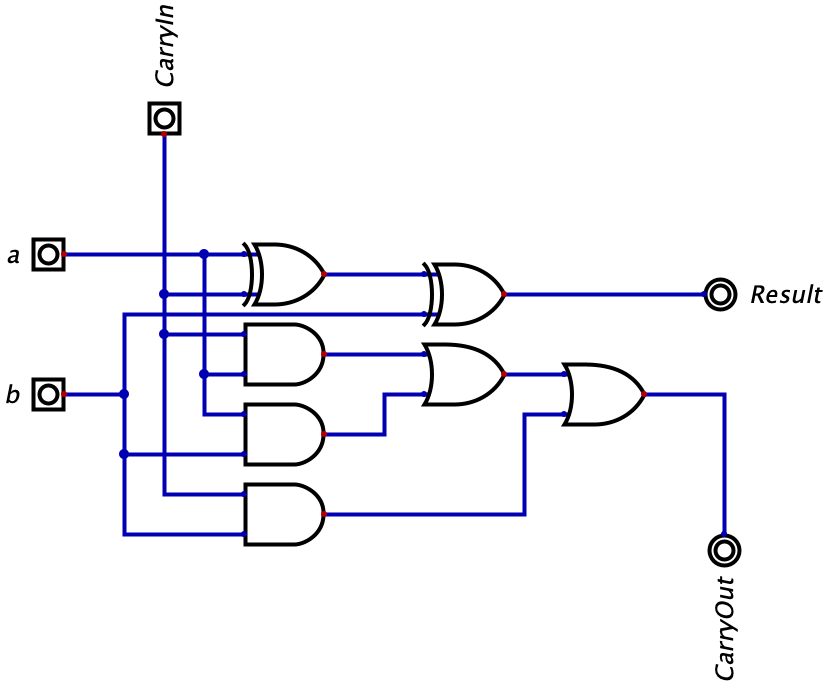
\includegraphics[width=0.5\textwidth]{assets/full_adder.png}
    \caption{Full-Adder Circuit}
    \label{fig:full_adder}
    \end{figure}

    \begin{figure}[h!]
        \centering
        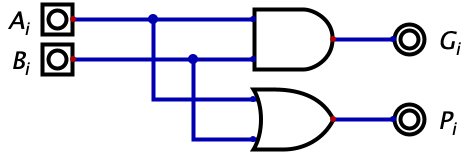
\includegraphics[width=0.5\textwidth]{assets/generate_gp.png}
        \caption{GP Generator Circuit}
        \label{fig:gp_generator}
        \end{figure}

\begin{figure*}[h!]
    \centering
    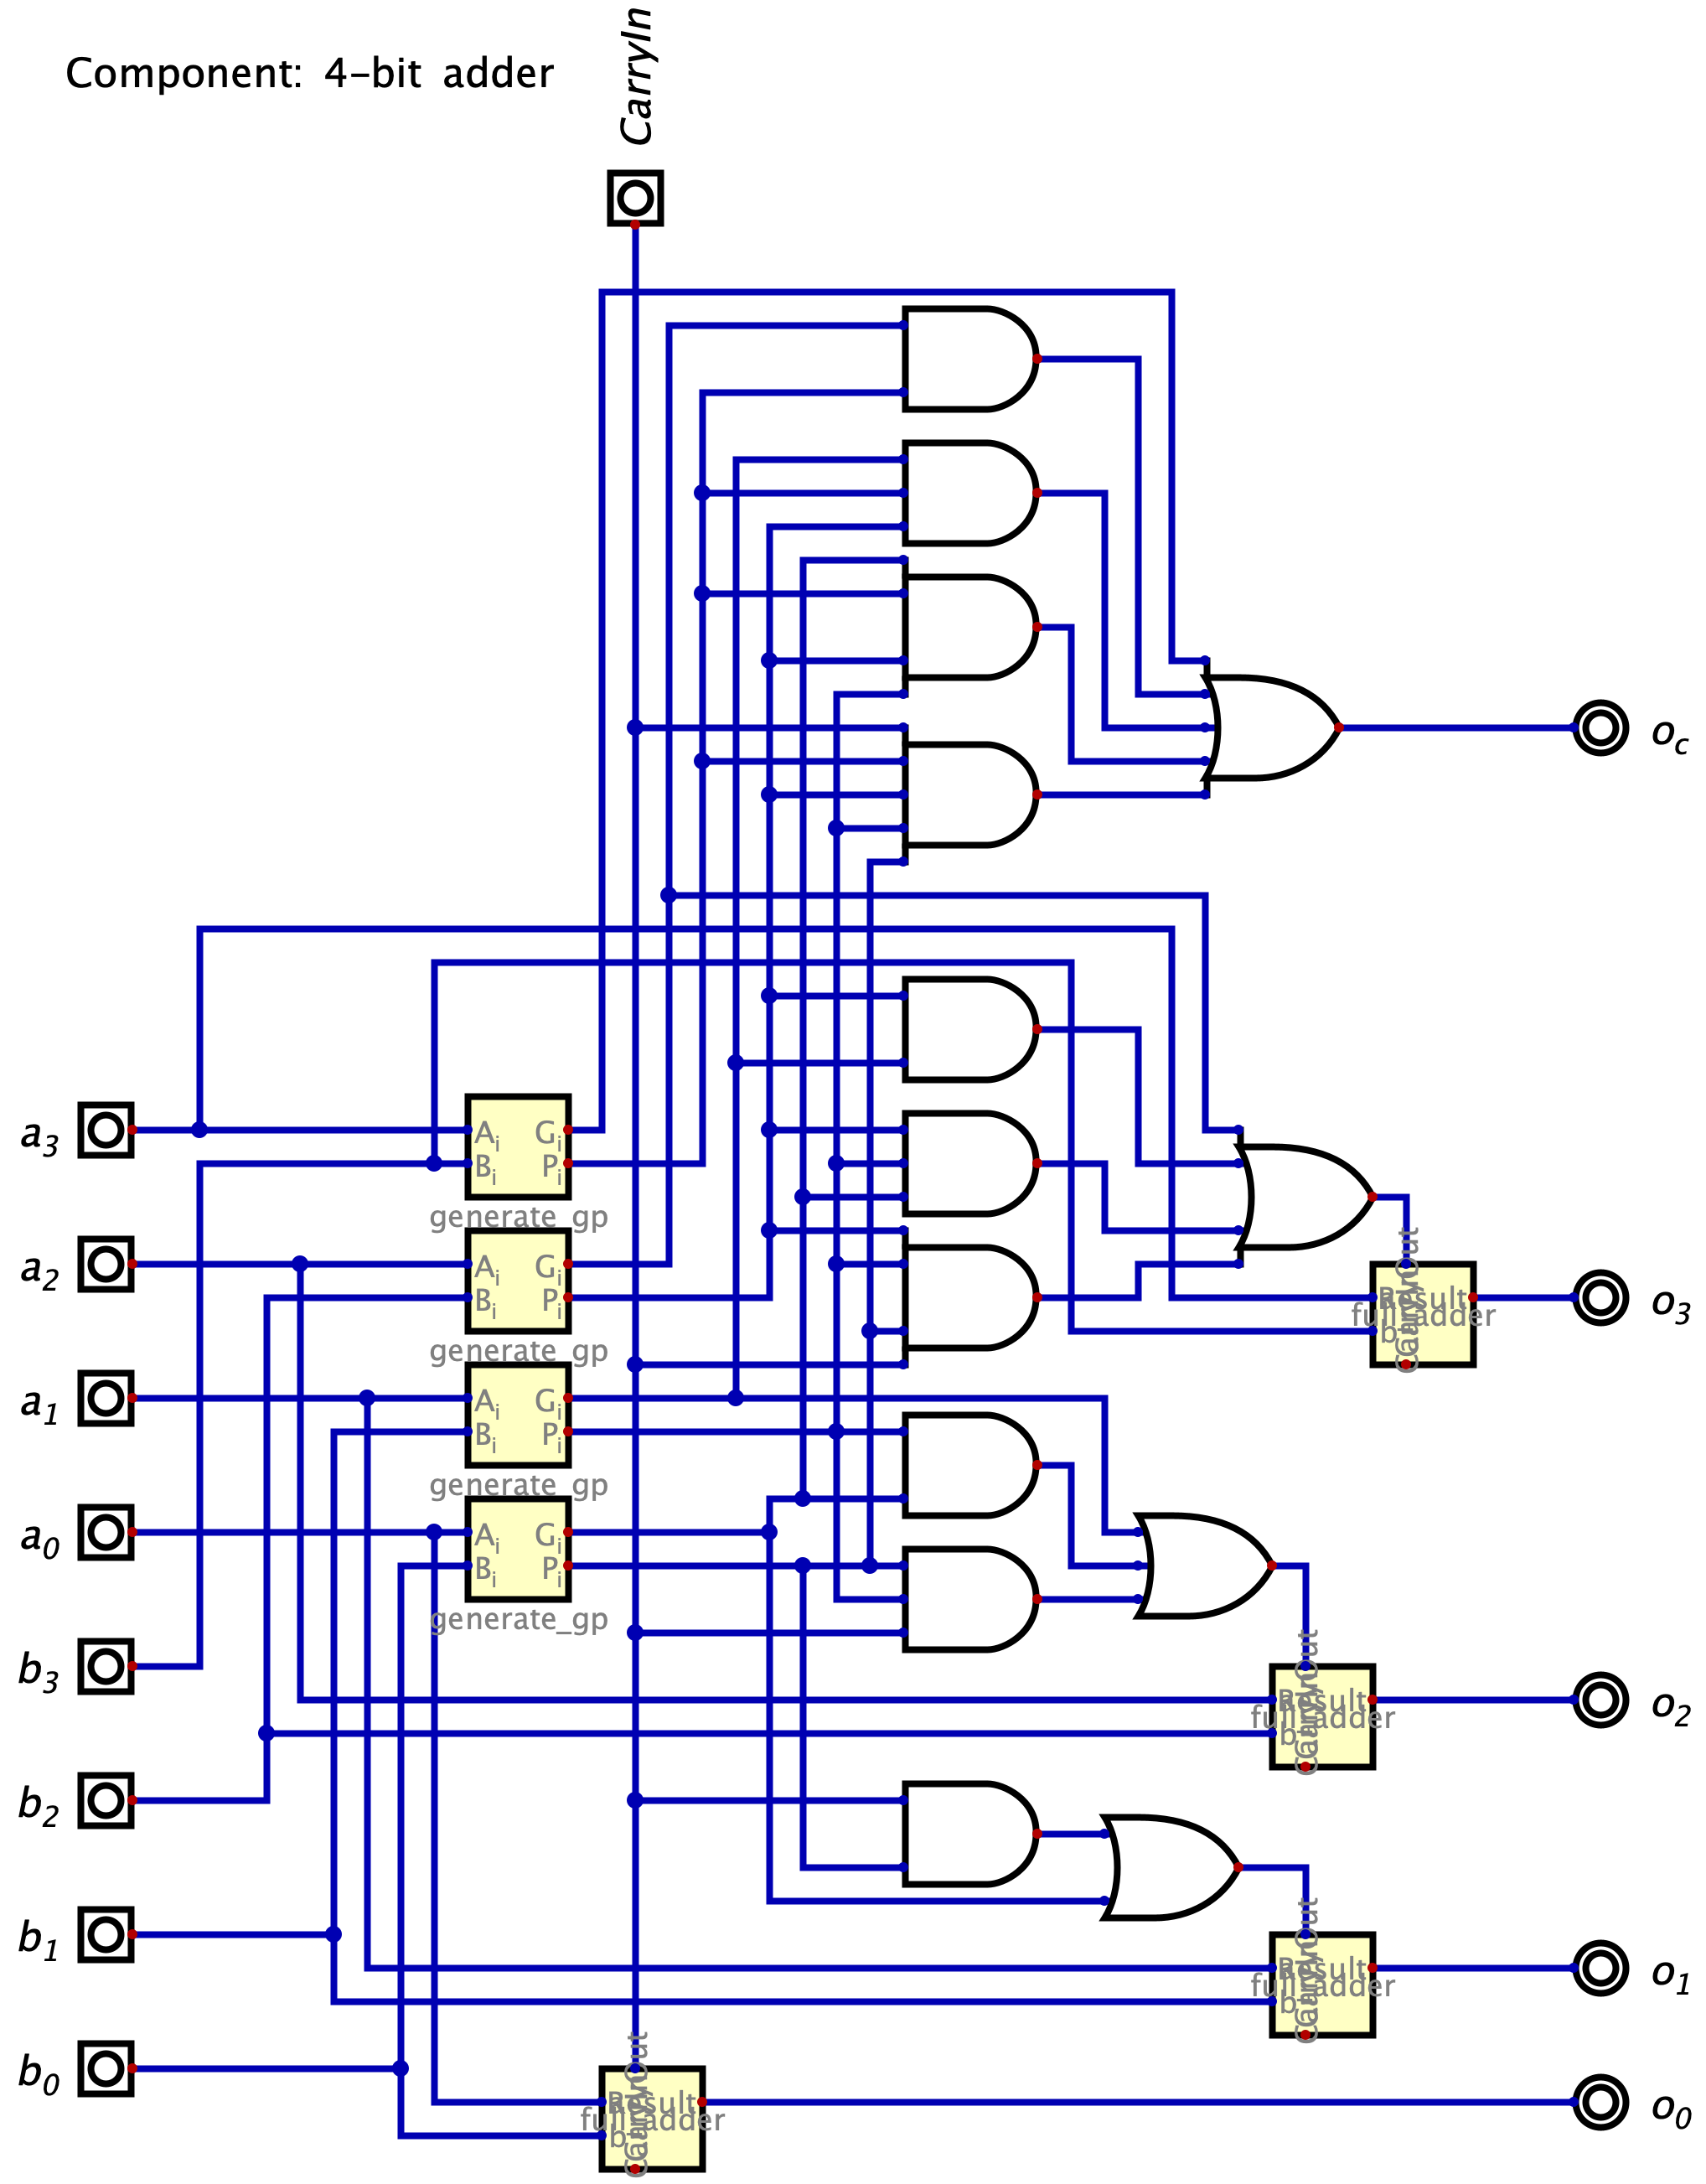
\includegraphics[width=\textwidth]{assets/adder_4bits.png}
    \caption{4-bit Lookahead Carry Adder}
    \label{fig:lca}
    \end{figure*}

    \begin{figure*}[h!]
        \centering
        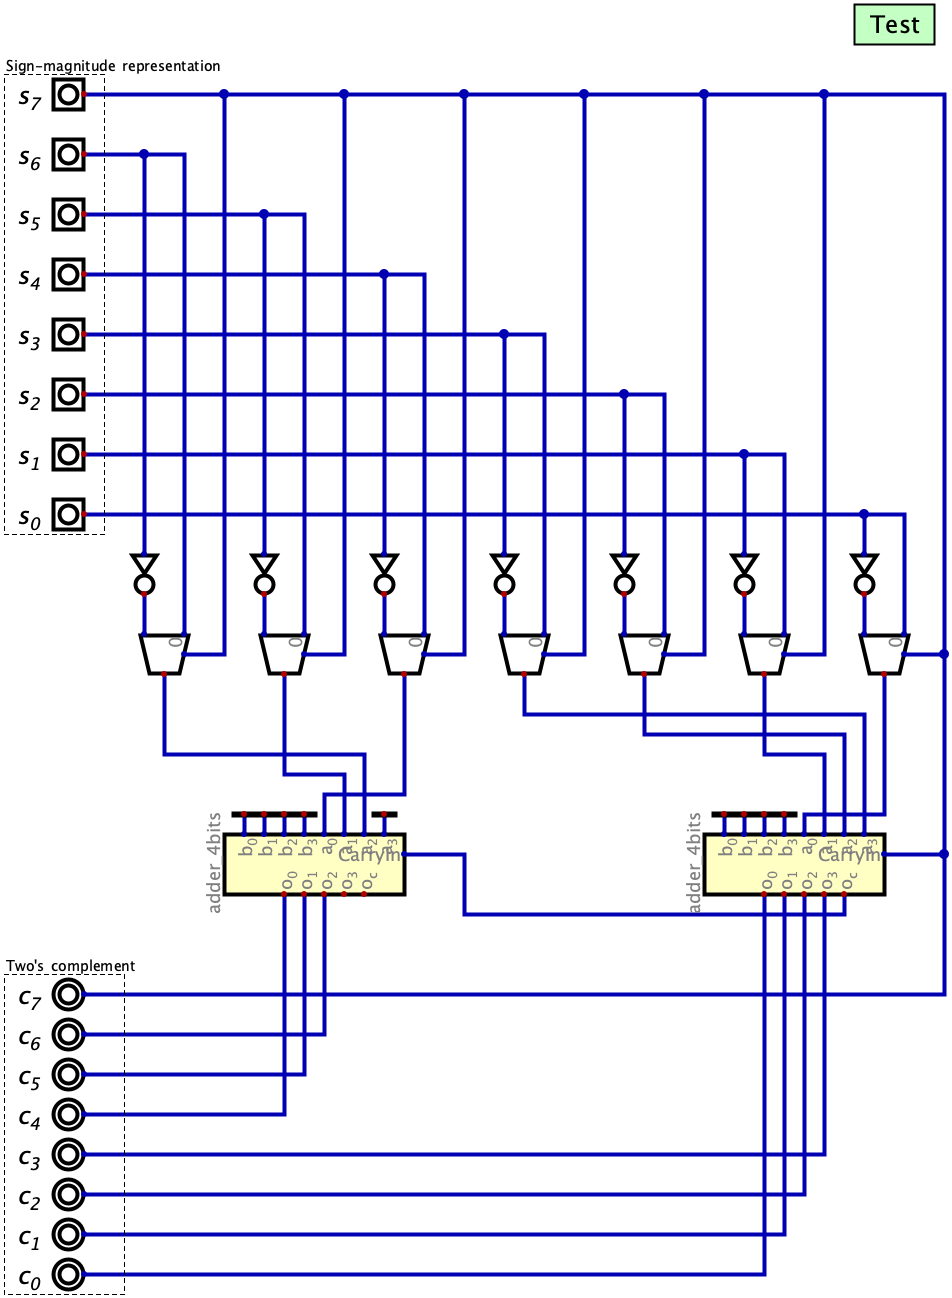
\includegraphics[width=\textwidth]{assets/twos_complement_dq.png}
        \caption{8-bit Two's Complement Circuit (Divide and Conquer Method)}
        \label{fig:tc-dq}
        \end{figure*}
    
\subsection{Question 4}

For a 8-bit adder, to calculate the depth and complexity of the circuit, we divide the circuit into two parts:
\begin{enumerate}
    \item In the \textbf{inversion stage}, all components are inversed simultaneously, thus depth is 1 and amount of NOT gates required is 7.
    \item In the \textbf{addition stage}, the two 4-bit lookahead carry adder one after another. They are connected in series.
          For a single 4-bit lookahead, the number of gates utilized is:
          \begin{equation}
            \underbrace{4 \time 2}_{\text{GP Generator}} + \underbrace{4 \times 7}_{\text{Full Adder}} + \underbrace{14}_{\text{In the middle layer}} = 46 
          \end{equation} 
          And the depth is:
          \begin{equation}
            \underbrace{1}_{\text{GP Generator}} + \underbrace{2}_{\text{In the middle layer}}  =3 
          \end{equation}

    \item Since there are two lookahead carry adder, the total depth is
     \begin{equation}
        1 + 3 \times 2 = 7
     \end{equation}
     and number of gates utilized is:
     \begin{equation}
        7 + 46 \times 2 = 100
     \end{equation}
\end{enumerate}

\end{document}
